%%%%%%%%%%%%%%%%%%%%%%%%%%%%%%%%%%%%%%%%%%%%%%%%%%%%%%%%%%%%%%%%%%%%
%% I, the copyright holder of this work, release this work into the
%% public domain. This applies worldwide. In some countries this may
%% not be legally possible; if so: I grant anyone the right to use
%% this work for any purpose, without any conditions, unless such
%% conditions are required by law.
%%%%%%%%%%%%%%%%%%%%%%%%%%%%%%%%%%%%%%%%%%%%%%%%%%%%%%%%%%%%%%%%%%%%

% This theme was based on fibeamer theme 
% If you found any bugs please contact @karlosos
% This repository is hosted on github https://github.com/karlosos/zut-fibeamer/

\documentclass{beamer}
\usetheme[faculty=wi]{./fibeamer}
\usepackage[utf8]{inputenc}
\usepackage[
  main=polish,
  polish
]{babel}

\title{Aula 3  - Rotas NodeJs}
\subtitle{Tópicos especiais em Sistemas}
\author{Prof. Juliana Costa Silva - juliana.silva@up.edu.br}

\usepackage{ragged2e}  % `\justifying` text
\usepackage{booktabs}  % Tables
\usepackage{tabularx}
\usepackage{tikz}      % Diagrams
\usetikzlibrary{calc, shapes, backgrounds}
\usepackage{amsmath, amssymb}
\usepackage{url}       % `\url`s
\usepackage{listings}  % Code listings
\frenchspacing
\begin{document}

%------------------------------------------------------------------------
  \frame[c]{\maketitle}
      \begin{frame}<beamer>
      \frametitle{O que veremos hoje}
      \tableofcontents
    \end{frame}
%------------------------------------------------------------------------
    \section{Revendo...}
    \begin{frame}{Revendo...}{O que já aprendemos?}
      
      \begin{itemize}
            \item Criamos um projeto node;
            \item Configuramos a porta do através do arquivo \textbf{index.js};
            \item Definimos o get de nosso aplicação;
       \end{itemize}
     \end{frame}
%------------------------------------------------------------------------
%    \begin{frame}[label=lists]{Ferramentas e tecnologias}
%      \begin{columns}[onlytextwidth]
%        \column{.5\textwidth}
%          \begin{itemize}
%            \item NodeJS \textcolor{gray}{(instalar até a próxima aula)}
%            \item VSCode \textcolor{gray}{(ou outra IDE da preferência do aluno)}
%            \item AngularJS 
%          \end{itemize}
%        \column{.5\textwidth}
%            
\includegraphics[width=55mm]{resources/aula1_4.png}
%      \end{columns}
%    \end{frame}
%------------------------------------------------------------------------
\section{Introdução}
\begin{frame}[label=proof]{O projeto da disciplina}
	\begin{itemize}
	\item Faremos um sistema de controle financeiro pessoal;
	\item Este sistema deve ter:
	\begin{itemize}
	\item Registro de gastos;
	\item Login de usuários;
	\item Registro de renda (salários - comissões - negócios);
	\item Registro de cartões de créditos;
	\item Registro de contas bancárias;
	\end{itemize}
	\end{itemize}
    \end{frame}
%------------------------------------------------------------------------
\section{Rotas}
    \begin{frame}[label=lists]{Rotas}
    \begin{exampleblock}{O que são rotas?}
        	\begin{itemize}
	\item Rotas são as configurações dadas aos caminhos percorridos no seu sistema;
	\item Por exemplo, você deseja ver os gastos realizados, qual seria o caminho?
	\item seusite/gastos
        	\end{itemize}
      \end{exampleblock}
            %
\includegraphics[width=90mm]{resources/aula1_5.png}\\
            %\tiny{\textbf{Fonte:} \cite{ich2021}}
    \end{frame}
%------------------------------------------------------------------------
    \begin{frame}[label=lists]{Configurando rota}

% \begin{columns}[onlytextwidth]
%        \column{.5\textwidth}
     
         Vamos configurar a rota  \url{http://localhost:3000/gastos}.\\
          \vspace{0.5cm}
          Edite a \underline{linha 7} do arquivo \textbf{index.js}, conforme apresentado abaixo, após a edição inicie o servidor node e acesse o endereço configurado.
%
%        \column{.5\textwidth}

	            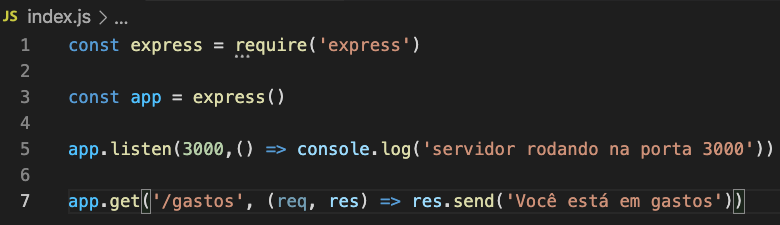
\includegraphics[width=110mm]{resources/aula3_1.png}\\
            \tiny{\textbf{Fonte:} O autor}

%      \end{columns}
    \end{frame}

 %------------------------------------------------------------------------
    \begin{frame}[label=lists]{package.json}
	O arquivo \textbf{package.json} contem todas as informações do nosso projeto, desde o nome, sua versão e scripts que podem ser executados até novos pacotes que poderemos instalar.\\
	\begin{exampleblock}{Editando package.json}
	\begin{itemize}
	\item Edite a propriedade scripts do arquivo (linha 6);
	\item Inclua um novo scrip, o start, e então poderá inserir o comando que quiser, como início do seu projeto. 

	\end{itemize}
	\end{exampleblock}

    \end{frame}
     %------------------------------------------------------------------------
    \begin{frame}[label=lists]{package.json}
		\begin{exampleblock}{Editando package.json}
	\begin{itemize}
	\item Ao invés de obrigarmos quem está acessando o servidor a escrever node index.js e diretório de instalação, padronizaremos que o arquivo de start realizará o comando \alert{node index.js}.
	\end{itemize}
	\end{exampleblock}
	 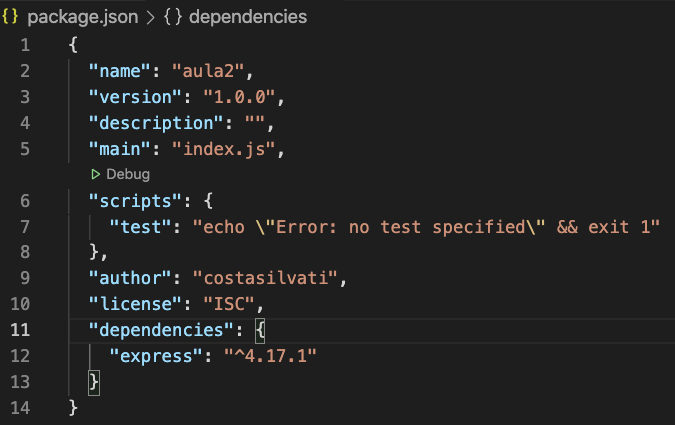
\includegraphics[width=80mm]{resources/aula3_2.png}\\
            \tiny{\textbf{Fonte:} O autor}

    \end{frame}
   
 %------------------------------------------------------------------------
    \begin{frame}[label=lists]{package.json}
		\begin{exampleblock}{Editando package.json}
	\begin{itemize}
	\item start realizará o comando \alert{node index.js}.
	\item O arquivo deve ficar como abaixo;
	\end{itemize}
	\end{exampleblock}
	 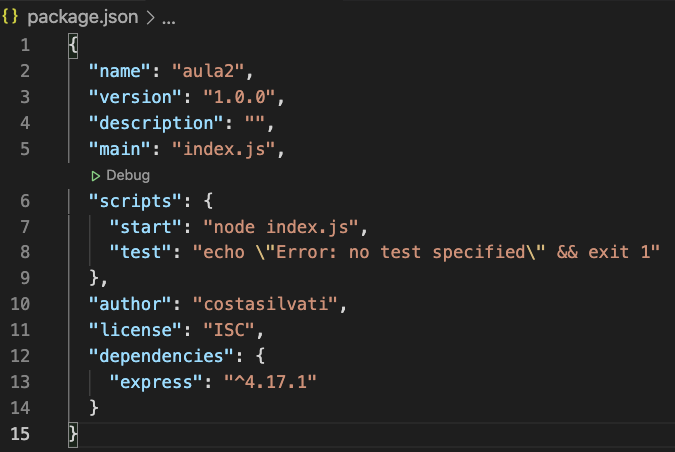
\includegraphics[width=80mm]{resources/aula3_3.png}\\
            \tiny{\textbf{Fonte:} O autor}

    \end{frame}
   
    %------------------------------------------------------------------------
    \begin{frame}[label=lists]{package.json}
		\begin{exampleblock}{Iniciando o projeto com npm}
	\begin{itemize}
	\item Agora seu projeto será iniciado no servidor através do comando
	\item \alert{npm start}
	\end{itemize}
	\end{exampleblock}
    \end{frame}
 %------------------------------------------------------------------------
 \section{nodemon}
\section{Ajustes no projeto}
    \begin{frame}[label=proof]{Reiniciar o servidor node}
	\begin{itemize}
	\item Para cada alteração que fazemos no projeto, precisamos para o servidor node com \alert{Ctrl + C};
	\item Iniciar o servidor novamente com o comando \alert{node index.js} para que ele carregue o projeto atualizado;
	\item Existe uma maneira melhor de fazer isso?
	\end{itemize}
    \end{frame}
 %------------------------------------------------------------------------
    \begin{frame}{Instalando o nodemon}
      \begin{columns}[onlytextwidth]
        \column{.5\textwidth}
         Pare o servidor.
        
          \vspace{0.5cm}
	Instale o nodemon
        \column{.5\textwidth}
            \pause
            \begin{itemize}
		\item Comando: \alert{npm install -- save-dev nodemon};
		\item Feito isso, em nosso script de start não precisamos mais ter node index.js, mas sim nodemon index.js. No console executaremos o npm start, e para restartar os servidor só precisamos ativar o comando start.
	\end{itemize}
      \end{columns}
      Observe as dependências criadas no arquivo \textbf{package.json}.
    \end{frame}
   
%------------------------------------------------------------------------
% \subsection{Referências}
%    \begin{frame}{Referências}%[allowframebreaks]
%\frametitle{Referências}
%\small
%\begin{center}
%\tiny
%\bibliographystyle{apalike}
%\bibliography{./ref_aula}
%\end{center}
%\end{frame}
  
\end{document}
